% Options for packages loaded elsewhere
\PassOptionsToPackage{unicode}{hyperref}
\PassOptionsToPackage{hyphens}{url}
\PassOptionsToPackage{dvipsnames,svgnames,x11names}{xcolor}
%
\documentclass[
  singlecolumn]{report}

\usepackage{amsmath,amssymb}
\usepackage{iftex}
\ifPDFTeX
  \usepackage[T1]{fontenc}
  \usepackage[utf8]{inputenc}
  \usepackage{textcomp} % provide euro and other symbols
\else % if luatex or xetex
  \usepackage{unicode-math}
  \defaultfontfeatures{Scale=MatchLowercase}
  \defaultfontfeatures[\rmfamily]{Ligatures=TeX,Scale=1}
\fi
\usepackage[]{libertinus}
\ifPDFTeX\else  
    % xetex/luatex font selection
\fi
% Use upquote if available, for straight quotes in verbatim environments
\IfFileExists{upquote.sty}{\usepackage{upquote}}{}
\IfFileExists{microtype.sty}{% use microtype if available
  \usepackage[]{microtype}
  \UseMicrotypeSet[protrusion]{basicmath} % disable protrusion for tt fonts
}{}
\makeatletter
\@ifundefined{KOMAClassName}{% if non-KOMA class
  \IfFileExists{parskip.sty}{%
    \usepackage{parskip}
  }{% else
    \setlength{\parindent}{0pt}
    \setlength{\parskip}{6pt plus 2pt minus 1pt}}
}{% if KOMA class
  \KOMAoptions{parskip=half}}
\makeatother
\usepackage{xcolor}
\usepackage[top=30mm,left=20mm,heightrounded]{geometry}
\setlength{\emergencystretch}{3em} % prevent overfull lines
\setcounter{secnumdepth}{-\maxdimen} % remove section numbering
% Make \paragraph and \subparagraph free-standing
\ifx\paragraph\undefined\else
  \let\oldparagraph\paragraph
  \renewcommand{\paragraph}[1]{\oldparagraph{#1}\mbox{}}
\fi
\ifx\subparagraph\undefined\else
  \let\oldsubparagraph\subparagraph
  \renewcommand{\subparagraph}[1]{\oldsubparagraph{#1}\mbox{}}
\fi


\providecommand{\tightlist}{%
  \setlength{\itemsep}{0pt}\setlength{\parskip}{0pt}}\usepackage{longtable,booktabs,array}
\usepackage{calc} % for calculating minipage widths
% Correct order of tables after \paragraph or \subparagraph
\usepackage{etoolbox}
\makeatletter
\patchcmd\longtable{\par}{\if@noskipsec\mbox{}\fi\par}{}{}
\makeatother
% Allow footnotes in longtable head/foot
\IfFileExists{footnotehyper.sty}{\usepackage{footnotehyper}}{\usepackage{footnote}}
\makesavenoteenv{longtable}
\usepackage{graphicx}
\makeatletter
\def\maxwidth{\ifdim\Gin@nat@width>\linewidth\linewidth\else\Gin@nat@width\fi}
\def\maxheight{\ifdim\Gin@nat@height>\textheight\textheight\else\Gin@nat@height\fi}
\makeatother
% Scale images if necessary, so that they will not overflow the page
% margins by default, and it is still possible to overwrite the defaults
% using explicit options in \includegraphics[width, height, ...]{}
\setkeys{Gin}{width=\maxwidth,height=\maxheight,keepaspectratio}
% Set default figure placement to htbp
\makeatletter
\def\fps@figure{htbp}
\makeatother
\newlength{\cslhangindent}
\setlength{\cslhangindent}{1.5em}
\newlength{\csllabelwidth}
\setlength{\csllabelwidth}{3em}
\newlength{\cslentryspacingunit} % times entry-spacing
\setlength{\cslentryspacingunit}{\parskip}
\newenvironment{CSLReferences}[2] % #1 hanging-ident, #2 entry spacing
 {% don't indent paragraphs
  \setlength{\parindent}{0pt}
  % turn on hanging indent if param 1 is 1
  \ifodd #1
  \let\oldpar\par
  \def\par{\hangindent=\cslhangindent\oldpar}
  \fi
  % set entry spacing
  \setlength{\parskip}{#2\cslentryspacingunit}
 }%
 {}
\usepackage{calc}
\newcommand{\CSLBlock}[1]{#1\hfill\break}
\newcommand{\CSLLeftMargin}[1]{\parbox[t]{\csllabelwidth}{#1}}
\newcommand{\CSLRightInline}[1]{\parbox[t]{\linewidth - \csllabelwidth}{#1}\break}
\newcommand{\CSLIndent}[1]{\hspace{\cslhangindent}#1}

\usepackage{booktabs}
\usepackage{longtable}
\usepackage{array}
\usepackage{multirow}
\usepackage{wrapfig}
\usepackage{float}
\usepackage{colortbl}
\usepackage{pdflscape}
\usepackage{tabu}
\usepackage{threeparttable}
\usepackage{threeparttablex}
\usepackage[normalem]{ulem}
\usepackage{makecell}
\usepackage{xcolor}
\usepackage{cancel}
\makeatletter
\makeatother
\makeatletter
\makeatother
\makeatletter
\@ifpackageloaded{caption}{}{\usepackage{caption}}
\AtBeginDocument{%
\ifdefined\contentsname
  \renewcommand*\contentsname{Table of contents}
\else
  \newcommand\contentsname{Table of contents}
\fi
\ifdefined\listfigurename
  \renewcommand*\listfigurename{List of Figures}
\else
  \newcommand\listfigurename{List of Figures}
\fi
\ifdefined\listtablename
  \renewcommand*\listtablename{List of Tables}
\else
  \newcommand\listtablename{List of Tables}
\fi
\ifdefined\figurename
  \renewcommand*\figurename{Figure}
\else
  \newcommand\figurename{Figure}
\fi
\ifdefined\tablename
  \renewcommand*\tablename{Table}
\else
  \newcommand\tablename{Table}
\fi
}
\@ifpackageloaded{float}{}{\usepackage{float}}
\floatstyle{ruled}
\@ifundefined{c@chapter}{\newfloat{codelisting}{h}{lop}}{\newfloat{codelisting}{h}{lop}[chapter]}
\floatname{codelisting}{Listing}
\newcommand*\listoflistings{\listof{codelisting}{List of Listings}}
\makeatother
\makeatletter
\@ifpackageloaded{caption}{}{\usepackage{caption}}
\@ifpackageloaded{subcaption}{}{\usepackage{subcaption}}
\makeatother
\makeatletter
\@ifpackageloaded{tcolorbox}{}{\usepackage[skins,breakable]{tcolorbox}}
\makeatother
\makeatletter
\@ifundefined{shadecolor}{\definecolor{shadecolor}{rgb}{.97, .97, .97}}
\makeatother
\makeatletter
\makeatother
\makeatletter
\makeatother
\ifLuaTeX
  \usepackage{selnolig}  % disable illegal ligatures
\fi
\IfFileExists{bookmark.sty}{\usepackage{bookmark}}{\usepackage{hyperref}}
\IfFileExists{xurl.sty}{\usepackage{xurl}}{} % add URL line breaks if available
\urlstyle{same} % disable monospaced font for URLs
\hypersetup{
  pdftitle={Effect of extraversion on Multi-dimensionsal well-being},
  pdfkeywords={measurement},
  colorlinks=true,
  linkcolor={blue},
  filecolor={Maroon},
  citecolor={Blue},
  urlcolor={Blue},
  pdfcreator={LaTeX via pandoc}}

\title{Effect of extraversion on Multi-dimensionsal well-being}
\author{}
\date{2023-07-09}

\begin{document}
\maketitle
\begin{abstract}
We combine national longitudinal time-series data with the potential
outcomes framework to estimate the causal effects of extraversion on
multidimensional well-being. We find evidence for a one-year causal
effect of extraversion on psychological and social well-being, but not
on health.
\end{abstract}
\ifdefined\Shaded\renewenvironment{Shaded}{\begin{tcolorbox}[sharp corners, enhanced, breakable, boxrule=0pt, borderline west={3pt}{0pt}{shadecolor}, interior hidden, frame hidden]}{\end{tcolorbox}}\fi

\listoffigures
\listoftables
\hypertarget{introduction}{%
\section{Introduction}\label{introduction}}

There is correlational research that showing that extraversion is
correlated with well-being. Evidence for causality, however, is scarce.

\hypertarget{method}{%
\section{Method}\label{method}}

\begin{itemize}
\tightlist
\item
  We apply doubly-robust estimators to longitudinal data from the the
  New Zealand Attitudes and Values Study
  (\protect\hyperlink{ref-sibley2021}{Chris G. Sibley 2021}) waves
  10-12.
\item
  We measure extraversion using the Mini-IPIP6
  (\protect\hyperlink{ref-sibley2011}{Chris G. Sibley et al. 2011})
\item
  To assess causality we require a causal estimand: ``what would happen
  if?''
\item
  We use the target-trial framework following Miguel A. Hernán et al.
  (\protect\hyperlink{ref-hernuxe1n2016}{2016}) to consider the
  hypothetical causal effect of shifting the population from the second
  quartile on extraversion to the fourth quartile
  (\protect\hyperlink{ref-hernuxe1n2022}{Miguel A. Hernán, Wang, and
  Leaf 2022}; \protect\hyperlink{ref-bulbulia2022}{Bulbulia 2022};
  \protect\hyperlink{ref-hernan2023}{Hernan and Robins 2023}). This
  estimand in interesting because it has practical implications. If we
  could intervene on people with relatively low extraversion to
  relatively high extra-version, what would be the outcome across
  multi-dimensional well-being?
\item
  We consider multi-dimensional well-being following VanderWeele,
  Mathur, and Chen (\protect\hyperlink{ref-vanderweele2020}{2020})
  outcome-wide model, to improve scientific understanding while avoiding
  selectivity in measures of well-being.
\end{itemize}

\hypertarget{selection-criteria}{%
\subsection{Selection criteria}\label{selection-criteria}}

\begin{itemize}
\tightlist
\item
  Enrolled in NZAVS in 2018 and 2019.
\item
  Responded to extraversion items in 2018 and 2019.
\item
  Could be lost to follow up in 2020 (missing data multiply imputed).
\item
  Missing data permitted in all other indicators (multiply imputed).
\end{itemize}

Figure~\ref{fig-outcomewide-dag} presents the three-wave design for
causal inference. By including indicators of the both the exposure and
outcome at baseline, any unmeasured confounder of the exposure (+1
baseline) and outcome (+2 baseline) would need to be orthogonal to the
baseline indicators. Although our approach offers a powerful means for
controlling unmeasured confounding, because we cannot ensure balance, we
peform sensitivity analysis by evaluating E-values. E-values represent
the minimum strength of association on the Risk-Ratio scale that an
unmeasured confounder would need to have with both treatment and outcome
in order to explain the observed effect estimates conditional on
measured covariates
(\protect\hyperlink{ref-vanderweele2017}{\textbf{vanderweele2017?}}).
E-values for all outcomes are reported in the tables and graphs below.

\begin{figure}

{\centering \includegraphics[width=0.8\textwidth,height=\textheight]{extroversion_files/figure-pdf/fig-outcomewide-dag-1.pdf}

}

\caption{\label{fig-outcomewide-dag}Causal graph: three-wave panel
design with selection bias}

\end{figure}

\hypertarget{selection-bias}{%
\subsection{Selection Bias}\label{selection-bias}}

To avoid selection bias from non-response and attrition bias, we
multiply imputed missing data as presented in Figure~\ref{fig-dag}. We
perform multiple imputation \emph{separately} within each qauartile of
extraversion, and combine the imputations after modelling missingness
conditional on the observed covariates (see:
(\protect\hyperlink{ref-zhang2023}{Zhang et al. 2023};
\protect\hyperlink{ref-westreich2015}{Westreich et al. 2015})). We
implement multiple imputation using the \texttt{mice} package in R
(\protect\hyperlink{ref-vanbuuren2018}{Van Buuren 2018}). We imputed 10
x missing data sets which were passed separately to the the
\texttt{MatchThem} and \texttt{WeightIt} packages to obtain exposure
weights (akin to propensity scores).

\begin{figure}

{\centering 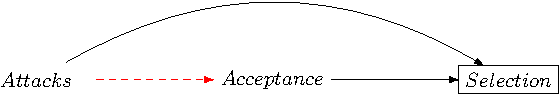
\includegraphics[width=0.8\textwidth,height=\textheight]{extroversion_files/figure-pdf/fig-dag-1.pdf}

}

\caption{\label{fig-dag}Causal graph shows potential for selection bias
from loss to follow up or non-response. To address this, we multiply
impute missing values conditional on the assumption that missing values
are random conditional on the imputation model (MAR).}

\end{figure}

\hypertarget{assssing-positivity}{%
\subsection{Assssing positivity}\label{assssing-positivity}}

To evaluation causality requires that the intervention is plausible. Can
extraversion change? To evaluate this question we assessed evidence for
movement between different levels of extraversion between NZAVS wave 10
and wave 11.

\hypertarget{tbl-transition-factor}{}
\begin{longtable}[]{@{}ccccc@{}}
\caption{\label{tbl-transition-factor}Transition matrix for change
stability and change extraversion by quartiles. Labels show range on 1-7
response scale}\tabularnewline
\toprule\noalign{}
From & 1\_3 & 3\_3.75 & 3.75\_4.75 & 4.75\_7 \\
\midrule\noalign{}
\endfirsthead
\toprule\noalign{}
From & 1\_3 & 3\_3.75 & 3.75\_4.75 & 4.75\_7 \\
\midrule\noalign{}
\endhead
\bottomrule\noalign{}
\endlastfoot
1\_3 & 4779 & 1748 & 570 & 65 \\
3\_3.75 & 1799 & 2956 & 2158 & 297 \\
3.75\_4.75 & 633 & 2316 & 5564 & 2046 \\
4.75\_7 & 71 & 351 & 2277 & 6559 \\
\end{longtable}

The transition matrix in Table~\ref{tbl-transition-factor} describes the
shifts from one state of extraversion to another between the baseline
wave (nzavs wave 10) and the following wave (nzavs wave 11). The numbers
in the cells represent the number of individuals who transitioned from
one state (rows) to another (columns). For example, the cell in the
first row and third column shows the number of individuals who
transitioned from the first state (indicated by the left-most cell in
the row) to the third state (n=570). The top left cell shows the number
of individuals who remained in the first state (n = 4779). Here we find
that n=297 individuals moved from the second quartile to the fourth
quartile.

Note that it is possible to estimate different causal effects. For
example, we might have asked: ``What would the causal effect be in the
population if everyone were to move between the lowest quartile and the
third quartile?''

\textbf{Note to co-authors: we can pick a different Estimand.
Alternatively We could use a continuous estimand, or both. This is just
an example.}

\hypertarget{inverse-probability-of-treatment-weighting}{%
\subsection{Inverse Probability of Treatment
Weighting}\label{inverse-probability-of-treatment-weighting}}

We first identified covariates for which balance is required, following
VanderWeeles modified disjunctive cause criterion
(\protect\hyperlink{ref-vanderweele2019}{VanderWeele 2019};
\protect\hyperlink{ref-vanderweele2020}{VanderWeele, Mathur, and Chen
2020}).

We used the \texttt{WeightIt} package in R
(\protect\hyperlink{ref-greifer2023a}{Greifer 2023b}) to obtain weights
for the exposure model, where the exposure was modelled as a function of
all baseline covariates. We used the \texttt{cobalt} pack to assess the
reliability of weights (\protect\hyperlink{ref-greifer2023b}{Greifer
2023a}). These weights were further augmented by post-stratification
weights for the NZAVS on age, gender, and European ethnicity (see:
(\protect\hyperlink{ref-sibley2021}{Chris G. Sibley 2021})).

We doubly robust estimator in which all outcomes measured at time +2
(NZAVS wave 12) were regressed against the exposure measured at time +1
(NZAVS wave 11) \(\times\) all baseline covariates measured at time 0
(NZAVS wave 10). weights for the exposure modelled were included in the
weighted regression. This approach follows {``Agnostic Notes on
Regression Adjustments to Experimental Data: Reexamining Freedman{'}s
Critique''} (\protect\hyperlink{ref-agnostic}{n.d.}) to obtain the
confounding control that is sensitive to model misspecification for the
outcome model or the exposure model.

We used the \texttt{Clarify}
(\protect\hyperlink{ref-greifer2023}{Greifer et al. 2023};
\protect\hyperlink{ref-king2000}{King, Tomz, and Wittenberg 2000}) in R
(\protect\hyperlink{ref-rainey2023}{Rainey 2023}) to estimate standard
errors and confidence intervals.

We note that the confidence intervals for doubly robust models such as
ours tend to be wider (we prefer variance over bias).

Figure~\ref{fig-propensity-score-example} shows example of baseline
imbalance (Here, the reflective domain). All domains reveal strong
imbalence in the baseline covariates that predict the exposure.
Unsurpisingly, the strongest of these covariates pertain to the exposure
itself. This raises the important point that to access the incidence
effect, we must control for baseline exposure. Here we control both by
propensity score weighting (the exposure model) and regression
adjustment (the outcome model). We trimmed the weights of the exposure
model by .9975 to avoid very extreme weights while keeping the mean
difference in the adjusted values below .05, as recommended by
(\protect\hyperlink{ref-greifer2023}{Greifer et al. 2023}).
(\emph{Appendix to follow})

\begin{figure}

{\centering \includegraphics{extroversion_files/figure-pdf/fig-propensity-score-example-1.pdf}

}

\caption{\label{fig-propensity-score-example}Evidence for strong
imbalance of covariates at baseline.}

\end{figure}

\hypertarget{results}{%
\section{Results}\label{results}}

This set of results reports the hypothetical effect of intervening on
extraversion by setting the population to the lower quartile of
extraversion and increasinge extraversion to the third-quartile.
Outcomes are measured one-year after this hypothetical intervention.

\hypertarget{effects-on-health}{%
\subsection{Effects on health}\label{effects-on-health}}

\begin{figure}

{\centering 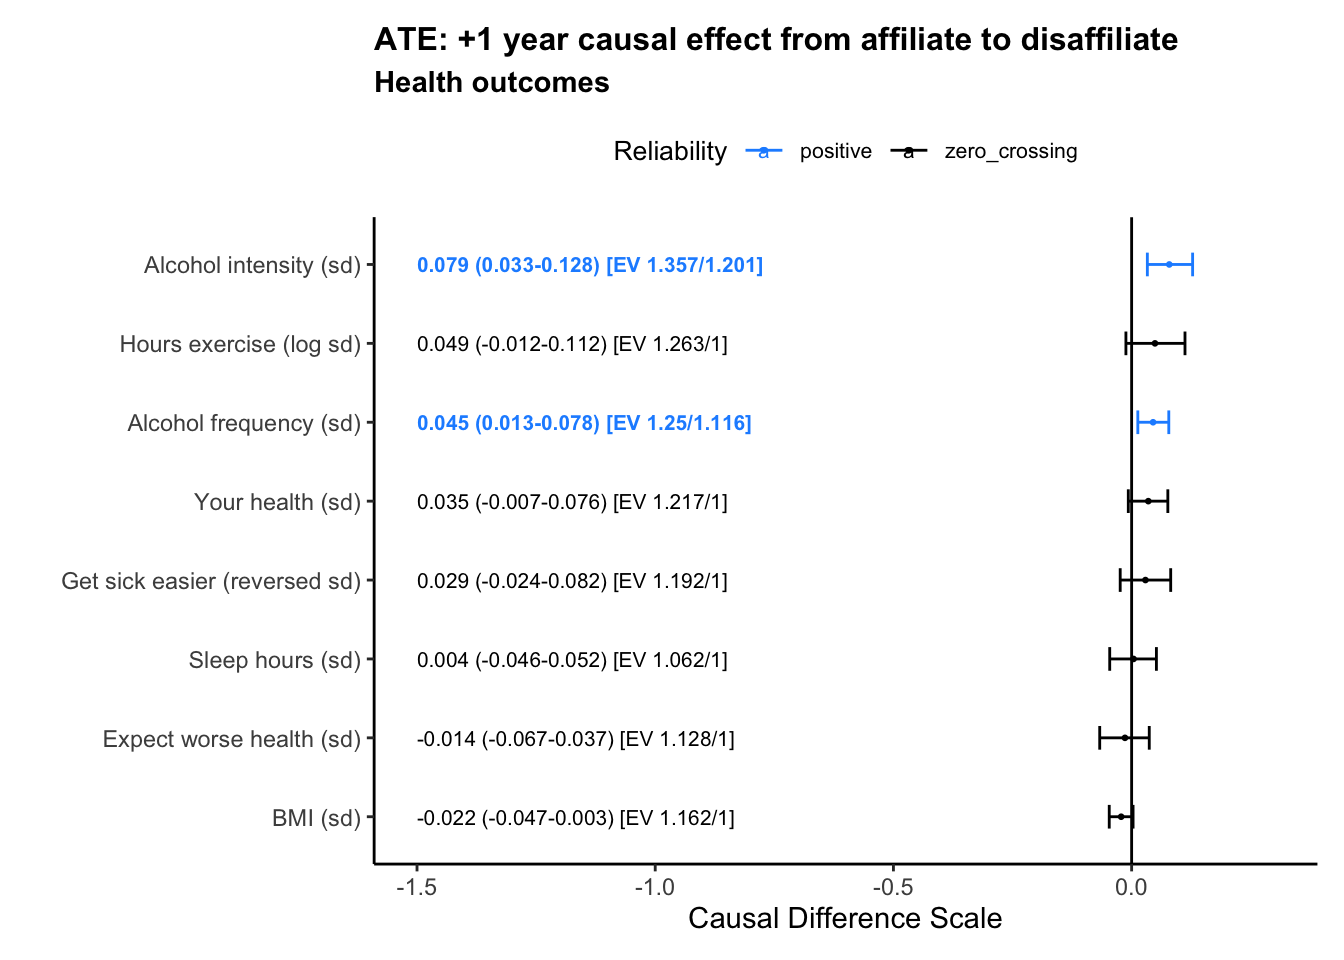
\includegraphics{extroversion_files/figure-pdf/fig-results-health-1.pdf}

}

\caption{\label{fig-results-health}Causal effects of extraversion gain
on reported physical health}

\end{figure}

Figure Figure~\ref{fig-results-health} and \textbf{?@tbl-results-health}
present the Population Average Treatment Effect (PATE). This is the
expected difference in outcomes between treatment and control groups for
the New Zealand population for the +1 year outcomes after a change in
extraversion. We do not find evidence of causal effects across the
health outcomes.

The population Average Treatment Effect (PATE) represents the expected
difference in outcomes between treatment and control groups for the New
Zealand population.

For the outcome `SF Health expect worse health (sd)', the PATE causal
contrast is 0.031. The confidence interval ranges from -0.039 to 0.097.
The E-value for this outcome confirms the causal contrast is unreliable.

For the outcome `Alcohol intensity (sd)', the PATE causal contrast is
0.03. The confidence interval ranges from -0.018 to 0.08. The E-value
for this outcome confirms the causal contrast is unreliable.

For the outcome `SF health your health (sd)', the PATE causal contrast
is 0.027. The confidence interval ranges from -0.031 to 0.088. The
E-value for this outcome confirms the causal contrast is unreliable.

For the outcome `alcohol frequency (sd)', the PATE causal contrast is
0.018. The confidence interval ranges from -0.028 to 0.069. The E-value
for this outcome confirms the causal contrast is unreliable.

For the outcome `SF Health get sick easier (sd, reversed)', the PATE
causal contrast is 0.015. The confidence interval ranges from -0.05 to
0.08. The E-value for this outcome confirms the causal contrast is
unreliable.

For the outcome `Hours exercise (log sd)', the PATE causal contrast is
-0.002. The confidence interval ranges from -0.078 to 0.068. The E-value
for this outcome confirms the causal contrast is unreliable.

For the outcome `Hlth bmi (sd)', the PATE causal contrast is -0.024. The
confidence interval ranges from -0.06 to 0.012. The E-value for this
outcome confirms the causal contrast is unreliable.

For the outcome `Hlth sleep Hours (sd)', the PATE causal contrast is
-0.029. The confidence interval ranges from -0.088 to 0.033. The E-value
for this outcome confirms the causal contrast is unreliable.

We did not find an effect on smoking (risk ratio) ,the PATE causal risk
ratio 0.967 (0.700, 1.333), and the confidence interval crosses 1
(1.223/1).

\hypertarget{effects-on-embodied-well-being}{%
\subsection{Effects on embodied
well-being}\label{effects-on-embodied-well-being}}

\begin{figure}

{\centering 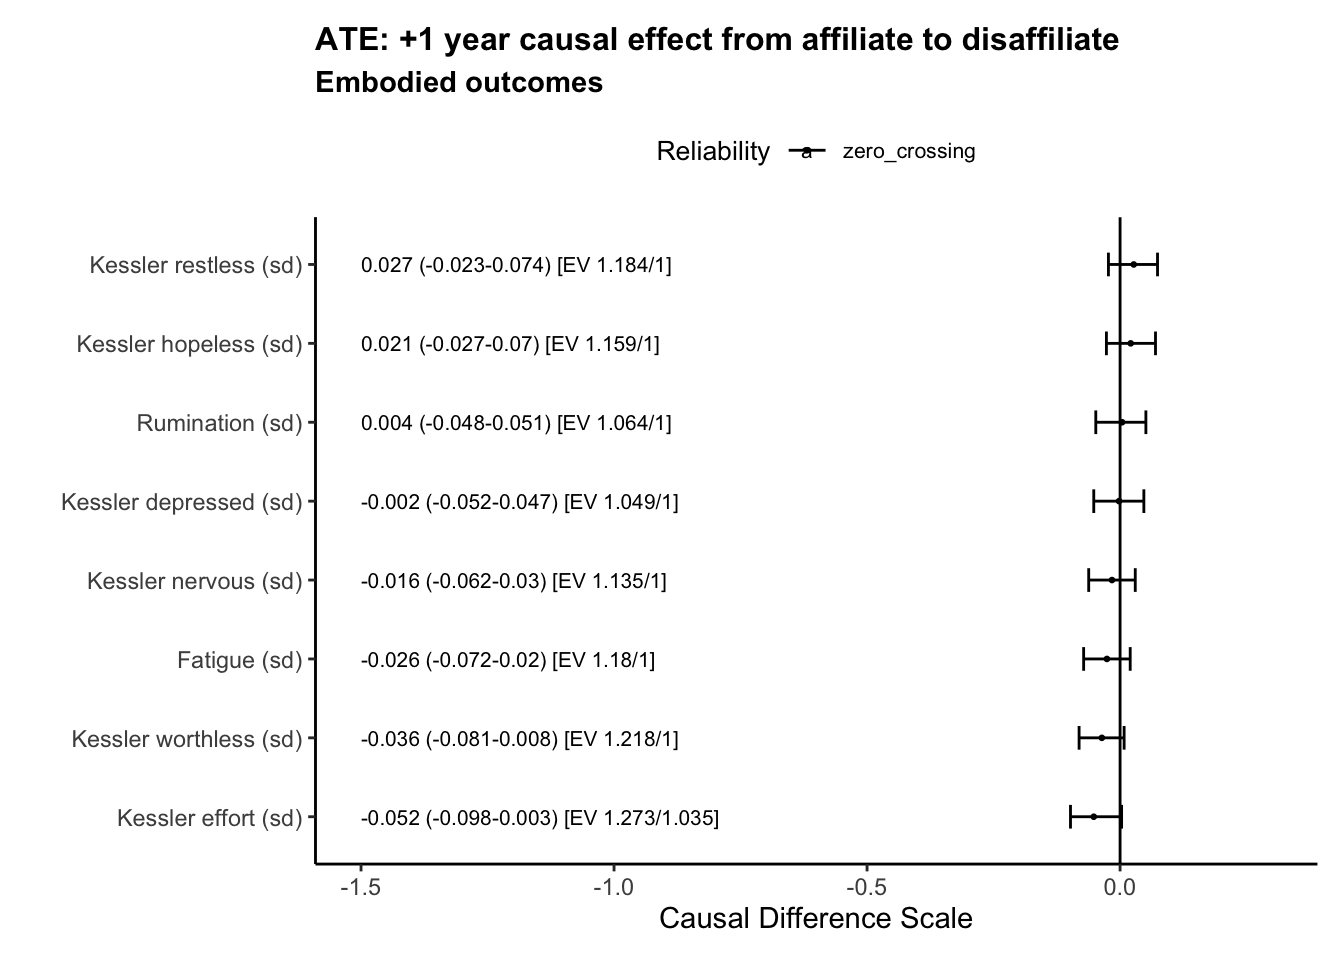
\includegraphics{extroversion_files/figure-pdf/fig-results-embodied-1.pdf}

}

\caption{\label{fig-results-embodied}Causal effects of extraversion gain
on embodied well-being}

\end{figure}

\hypertarget{tbl-results-embodied}{}
\begin{longtable}[]{@{}
  >{\raggedright\arraybackslash}p{(\columnwidth - 10\tabcolsep) * \real{0.3067}}
  >{\raggedleft\arraybackslash}p{(\columnwidth - 10\tabcolsep) * \real{0.2133}}
  >{\raggedleft\arraybackslash}p{(\columnwidth - 10\tabcolsep) * \real{0.1067}}
  >{\raggedleft\arraybackslash}p{(\columnwidth - 10\tabcolsep) * \real{0.1067}}
  >{\raggedleft\arraybackslash}p{(\columnwidth - 10\tabcolsep) * \real{0.1067}}
  >{\raggedleft\arraybackslash}p{(\columnwidth - 10\tabcolsep) * \real{0.1600}}@{}}
\caption{\label{tbl-results-embodied}Table of results for the embodied
well-being domain}\tabularnewline
\toprule\noalign{}
\begin{minipage}[b]{\linewidth}\raggedright
\end{minipage} & \begin{minipage}[b]{\linewidth}\raggedleft
E{[}Y(1){]}-E{[}Y(0){]}
\end{minipage} & \begin{minipage}[b]{\linewidth}\raggedleft
2.5 \%
\end{minipage} & \begin{minipage}[b]{\linewidth}\raggedleft
97.5 \%
\end{minipage} & \begin{minipage}[b]{\linewidth}\raggedleft
E\_Value
\end{minipage} & \begin{minipage}[b]{\linewidth}\raggedleft
E\_Val\_bound
\end{minipage} \\
\midrule\noalign{}
\endfirsthead
\toprule\noalign{}
\begin{minipage}[b]{\linewidth}\raggedright
\end{minipage} & \begin{minipage}[b]{\linewidth}\raggedleft
E{[}Y(1){]}-E{[}Y(0){]}
\end{minipage} & \begin{minipage}[b]{\linewidth}\raggedleft
2.5 \%
\end{minipage} & \begin{minipage}[b]{\linewidth}\raggedleft
97.5 \%
\end{minipage} & \begin{minipage}[b]{\linewidth}\raggedleft
E\_Value
\end{minipage} & \begin{minipage}[b]{\linewidth}\raggedleft
E\_Val\_bound
\end{minipage} \\
\midrule\noalign{}
\endhead
\bottomrule\noalign{}
\endlastfoot
kessler\_worthless (sd) & -0.1453 & -0.1999 & -0.0875 & 1.543 & 1.387 \\
Kessler nervous (sd) & -0.1124 & -0.1812 & -0.0500 & 1.453 & 1.257 \\
Kessler hopeless (sd) & -0.0722 & -0.1287 & -0.0141 & 1.337 & 1.132 \\
Rumination (sd) & -0.0808 & -0.1486 & -0.0133 & 1.363 & 1.123 \\
kessler restless (sd) & -0.0677 & -0.1302 & -0.0059 & 1.324 & 1.077 \\
Hlth fatigue (sd) & -0.0180 & -0.0844 & 0.0456 & 1.146 & 1.000 \\
Kessler depressed (sd) & -0.0256 & -0.0872 & 0.0384 & 1.179 & 1.000 \\
Kessler effort (sd) & -0.0510 & -0.1233 & 0.0176 & 1.271 & 1.000 \\
\end{longtable}

Figure~\ref{fig-results-embodied} and Table~\ref{tbl-results-embodied}
presents the Population Average Treatment Effect (PATE) for the embodied
domain. We find evidence for the causal effects of change in
extraversion (from the lowest quartile to the third quartile) on five of
the six Kessler-6 dimensions, with the strong effects on feelings of
worthlessless.

For the outcome `kessler\_worthless (sd)', the PATE causal contrast is
-0.145. The confidence interval ranges from -0.2 to -0.088. The E-value
for this outcome is 1.543, indicating reliable evidence for causality.

For the outcome `Kessler nervous (sd)', the PATE causal contrast is
-0.112. The confidence interval ranges from -0.181 to -0.05. The E-value
for this outcome is 1.453, indicating reliable evidence for causality.

For the outcome `Rumination (sd)', the PATE causal contrast is -0.081.
The confidence interval ranges from -0.149 to -0.013. The E-value for
this outcome is 1.363, indicating reliable evidence for causality.

For the outcome `Kessler hopeless (sd)', the PATE causal contrast is
-0.072. The confidence interval ranges from -0.129 to -0.014. The
E-value for this outcome is 1.337, indicating reliable evidence for
causality.

For the outcome `kessler restless (sd)', the PATE causal contrast is
-0.068. The confidence interval ranges from -0.13 to -0.006. The E-value
for this outcome is 1.324, indicating reliable evidence for causality.

For the outcome `Kessler effort (sd)', the PATE causal contrast is
-0.051. The confidence interval ranges from -0.123 to 0.018. The E-value
for this outcome confirms the causal contrast is unreliable.

For the outcome `Kessler depressed (sd)', the PATE causal contrast is
-0.026. The confidence interval ranges from -0.087 to 0.038. The E-value
for this outcome confirms the causal contrast is unreliable.

For the outcome `Hlth fatigue (sd)', the PATE causal contrast is -0.018.
The confidence interval ranges from -0.084 to 0.046. The E-value for
this outcome confirms the causal contrast is unreliable.

\hypertarget{effects-on-practical-well-being}{%
\subsection{Effects on practical
well-being}\label{effects-on-practical-well-being}}

\begin{figure}

{\centering \includegraphics{extroversion_files/figure-pdf/fig-results-practical-1.pdf}

}

\caption{\label{fig-results-practical}Causal effects of extraversion
gain on practical well-being}

\end{figure}

\hypertarget{tbl-results-practical}{}
\begin{longtable}[]{@{}
  >{\raggedright\arraybackslash}p{(\columnwidth - 10\tabcolsep) * \real{0.4348}}
  >{\raggedleft\arraybackslash}p{(\columnwidth - 10\tabcolsep) * \real{0.1739}}
  >{\raggedleft\arraybackslash}p{(\columnwidth - 10\tabcolsep) * \real{0.0870}}
  >{\raggedleft\arraybackslash}p{(\columnwidth - 10\tabcolsep) * \real{0.0870}}
  >{\raggedleft\arraybackslash}p{(\columnwidth - 10\tabcolsep) * \real{0.0870}}
  >{\raggedleft\arraybackslash}p{(\columnwidth - 10\tabcolsep) * \real{0.1304}}@{}}
\caption{\label{tbl-results-practical}Table of results for the practical
well-being domain}\tabularnewline
\toprule\noalign{}
\begin{minipage}[b]{\linewidth}\raggedright
\end{minipage} & \begin{minipage}[b]{\linewidth}\raggedleft
E{[}Y(1){]}-E{[}Y(0){]}
\end{minipage} & \begin{minipage}[b]{\linewidth}\raggedleft
2.5 \%
\end{minipage} & \begin{minipage}[b]{\linewidth}\raggedleft
97.5 \%
\end{minipage} & \begin{minipage}[b]{\linewidth}\raggedleft
E\_Value
\end{minipage} & \begin{minipage}[b]{\linewidth}\raggedleft
E\_Val\_bound
\end{minipage} \\
\midrule\noalign{}
\endfirsthead
\toprule\noalign{}
\begin{minipage}[b]{\linewidth}\raggedright
\end{minipage} & \begin{minipage}[b]{\linewidth}\raggedleft
E{[}Y(1){]}-E{[}Y(0){]}
\end{minipage} & \begin{minipage}[b]{\linewidth}\raggedleft
2.5 \%
\end{minipage} & \begin{minipage}[b]{\linewidth}\raggedleft
97.5 \%
\end{minipage} & \begin{minipage}[b]{\linewidth}\raggedleft
E\_Value
\end{minipage} & \begin{minipage}[b]{\linewidth}\raggedleft
E\_Val\_bound
\end{minipage} \\
\midrule\noalign{}
\endhead
\bottomrule\noalign{}
\endlastfoot
Perfectionism (sd) & -0.1665 & -0.2223 & -0.1109 & 1.600 & 1.449 \\
Power self nocontrol (sd) & -0.1588 & -0.2252 & -0.0941 & 1.579 &
1.399 \\
Emotion reg out control (sd) & -0.1492 & -0.2141 & -0.0894 & 1.554 &
1.381 \\
Power other control (sd) & -0.1379 & -0.1951 & -0.0803 & 1.523 &
1.362 \\
Selfesteem postive self (sd) & 0.1310 & 0.0719 & 0.1880 & 1.504 &
1.340 \\
Selfesteem failure (sd, reversed) & 0.1227 & 0.0677 & 0.1782 & 1.482 &
1.323 \\
Emotion reg hide neg emotions (sd) & -0.1283 & -0.1946 & -0.0604 & 1.497
& 1.304 \\
Selfesteem satself (sd) & 0.1058 & 0.0424 & 0.1682 & 1.435 & 1.244 \\
Bodysat (sd) & 0.0880 & 0.0256 & 0.1522 & 1.384 & 1.176 \\
Vengeful rumin (sd) & -0.0803 & -0.1363 & -0.0242 & 1.361 & 1.174 \\
Sexual satisfaction (sd) & 0.0281 & -0.0356 & 0.0950 & 1.189 & 1.000 \\
Self control have lots (sd) & -0.0287 & -0.0945 & 0.0363 & 1.191 &
1.000 \\
Self control wish more (sd, reversed) & 0.0162 & -0.0450 & 0.0734 &
1.138 & 1.000 \\
Emotion reg chang thinking to calm (sd) & 0.0087 & -0.0601 & 0.0759 &
1.097 & 1.000 \\
\end{longtable}

Figure~\ref{fig-results-practical} and Table~\ref{tbl-results-practical}
present the results for practical well-being.

For the outcome `Selfesteem postive self (sd)', the PATE causal contrast
is 0.131. The confidence interval ranges from 0.072 to 0.188. The
E-value for this outcome is 1.504, indicating reliable evidence for
causality.

For the outcome `Selfesteem failure (sd, reversed)', the PATE causal
contrast is 0.123. The confidence interval ranges from 0.068 to 0.178.
The E-value for this outcome is 1.482, indicating reliable evidence for
causality.

For the outcome `Selfesteem satself (sd)', the PATE causal contrast is
0.106. The confidence interval ranges from 0.042 to 0.168. The E-value
for this outcome is 1.435, indicating reliable evidence for causality.

For the outcome `Bodysat (sd)', the PATE causal contrast is 0.088. The
confidence interval ranges from 0.026 to 0.152. The E-value for this
outcome is 1.384, indicating reliable evidence for causality.

For the outcome `Sexual satisfaction (sd)', the PATE causal contrast is
0.028. The confidence interval ranges from -0.036 to 0.095. The E-value
for this outcome confirms the causal contrast is unreliable.

For the outcome `Self control wish more (sd, reversed)', the PATE causal
contrast is 0.016. The confidence interval ranges from -0.045 to 0.073.
The E-value for this outcome confirms the causal contrast is unreliable.

For the outcome `Emotion reg chang thinking to calm (sd)', the PATE
causal contrast is 0.009. The confidence interval ranges from -0.06 to
0.076. The E-value for this outcome confirms the causal contrast is
unreliable.

For the outcome `Self control have lots (sd)', the PATE causal contrast
is -0.029. The confidence interval ranges from -0.094 to 0.036. The
E-value for this outcome confirms the causal contrast is unreliable.

For the outcome `Vengeful rumin (sd)', the PATE causal contrast is
-0.08. The confidence interval ranges from -0.136 to -0.024. The E-value
for this outcome is 1.361, indicating reliable evidence for causality.

For the outcome `Emotion reg hide neg emotions (sd)', the PATE causal
contrast is -0.128. The confidence interval ranges from -0.195 to -0.06.
The E-value for this outcome is 1.497, indicating reliable evidence for
causality.

For the outcome `Power other control (sd)', the PATE causal contrast is
-0.138. The confidence interval ranges from -0.195 to -0.08. The E-value
for this outcome is 1.523, indicating reliable evidence for causality.

For the outcome `Emotion reg out control (sd)', the PATE causal contrast
is -0.149. The confidence interval ranges from -0.214 to -0.089. The
E-value for this outcome is 1.554, indicating reliable evidence for
causality.

For the outcome `Power self nocontrol (sd)', the PATE causal contrast is
-0.159. The confidence interval ranges from -0.225 to -0.094. The
E-value for this outcome is 1.579, indicating reliable evidence for
causality.

For the outcome `Perfectionism (sd)', the PATE causal contrast is
-0.166. The confidence interval ranges from -0.222 to -0.111. The
E-value for this outcome is 1.6, indicating reliable evidence for
causality.

\hypertarget{effects-on-reflective-well-being}{%
\subsection{Effects on reflective
well-being}\label{effects-on-reflective-well-being}}

\begin{figure}

{\centering \includegraphics{extroversion_files/figure-pdf/fig-results-reflective-well-being-1.pdf}

}

\caption{\label{fig-results-reflective-well-being}Causal effects of
extraversion gain on reflective well-being}

\end{figure}

\hypertarget{tbl-results-reflective}{}
\begin{longtable}[]{@{}
  >{\raggedright\arraybackslash}p{(\columnwidth - 10\tabcolsep) * \real{0.3200}}
  >{\raggedleft\arraybackslash}p{(\columnwidth - 10\tabcolsep) * \real{0.2133}}
  >{\raggedleft\arraybackslash}p{(\columnwidth - 10\tabcolsep) * \real{0.1067}}
  >{\raggedleft\arraybackslash}p{(\columnwidth - 10\tabcolsep) * \real{0.0933}}
  >{\raggedleft\arraybackslash}p{(\columnwidth - 10\tabcolsep) * \real{0.1067}}
  >{\raggedleft\arraybackslash}p{(\columnwidth - 10\tabcolsep) * \real{0.1600}}@{}}
\caption{\label{tbl-results-reflective}Table of results for the
reflective well-being domain}\tabularnewline
\toprule\noalign{}
\begin{minipage}[b]{\linewidth}\raggedright
\end{minipage} & \begin{minipage}[b]{\linewidth}\raggedleft
E{[}Y(1){]}-E{[}Y(0){]}
\end{minipage} & \begin{minipage}[b]{\linewidth}\raggedleft
2.5 \%
\end{minipage} & \begin{minipage}[b]{\linewidth}\raggedleft
97.5 \%
\end{minipage} & \begin{minipage}[b]{\linewidth}\raggedleft
E\_Value
\end{minipage} & \begin{minipage}[b]{\linewidth}\raggedleft
E\_Val\_bound
\end{minipage} \\
\midrule\noalign{}
\endfirsthead
\toprule\noalign{}
\begin{minipage}[b]{\linewidth}\raggedright
\end{minipage} & \begin{minipage}[b]{\linewidth}\raggedleft
E{[}Y(1){]}-E{[}Y(0){]}
\end{minipage} & \begin{minipage}[b]{\linewidth}\raggedleft
2.5 \%
\end{minipage} & \begin{minipage}[b]{\linewidth}\raggedleft
97.5 \%
\end{minipage} & \begin{minipage}[b]{\linewidth}\raggedleft
E\_Value
\end{minipage} & \begin{minipage}[b]{\linewidth}\raggedleft
E\_Val\_bound
\end{minipage} \\
\midrule\noalign{}
\endhead
\bottomrule\noalign{}
\endlastfoot
Gratitude (sd) & 0.1869 & 0.1376 & 0.2381 & 1.654 & 1.520 \\
PWI health (sd) & -0.0007 & -0.0570 & 0.0530 & 1.026 & 1.000 \\
PWI Relationships (sd) & 0.1127 & 0.0638 & 0.1635 & 1.454 & 1.309 \\
PWI security (sd) & 0.0387 & -0.0289 & 0.1039 & 1.229 & 1.000 \\
PWI standardliving (sd) & 0.0991 & 0.0361 & 0.1607 & 1.416 & 1.222 \\
Lifesat satlife (sd) & 0.0911 & 0.0373 & 0.1447 & 1.393 & 1.224 \\
Lifesat ideal (sd) & 0.0594 & 0.0001 & 0.1158 & 1.298 & 1.041 \\
Meaning purpose (sd) & 0.1265 & 0.0659 & 0.1846 & 1.492 & 1.322 \\
Meaning sense (sd) & 0.1284 & 0.0535 & 0.1926 & 1.497 & 1.296 \\
\end{longtable}

As indicated in Figure~\ref{fig-results-reflective-well-being} and
Table~\ref{tbl-results-reflective} we do not find evidence for reliable
effects of extraversion on personal security r personal health. However,
we find evidence for effects across all other dimensions of reflective
well-being.

\hypertarget{effects-social-well-being}{%
\subsection{Effects social well-being}\label{effects-social-well-being}}

\begin{figure}

{\centering \includegraphics{extroversion_files/figure-pdf/fig-results-social-wellbeing-1.pdf}

}

\caption{\label{fig-results-social-wellbeing}Causal effects of
extraversion gain on social well-being}

\end{figure}

\hypertarget{tbl-results-social}{}
\begin{longtable}[]{@{}
  >{\raggedright\arraybackslash}p{(\columnwidth - 10\tabcolsep) * \real{0.4000}}
  >{\raggedleft\arraybackslash}p{(\columnwidth - 10\tabcolsep) * \real{0.1882}}
  >{\raggedleft\arraybackslash}p{(\columnwidth - 10\tabcolsep) * \real{0.0941}}
  >{\raggedleft\arraybackslash}p{(\columnwidth - 10\tabcolsep) * \real{0.0824}}
  >{\raggedleft\arraybackslash}p{(\columnwidth - 10\tabcolsep) * \real{0.0941}}
  >{\raggedleft\arraybackslash}p{(\columnwidth - 10\tabcolsep) * \real{0.1412}}@{}}
\caption{\label{tbl-results-social}Table of results for the social
well-being domain}\tabularnewline
\toprule\noalign{}
\begin{minipage}[b]{\linewidth}\raggedright
\end{minipage} & \begin{minipage}[b]{\linewidth}\raggedleft
E{[}Y(1){]}-E{[}Y(0){]}
\end{minipage} & \begin{minipage}[b]{\linewidth}\raggedleft
2.5 \%
\end{minipage} & \begin{minipage}[b]{\linewidth}\raggedleft
97.5 \%
\end{minipage} & \begin{minipage}[b]{\linewidth}\raggedleft
E\_Value
\end{minipage} & \begin{minipage}[b]{\linewidth}\raggedleft
E\_Val\_bound
\end{minipage} \\
\midrule\noalign{}
\endfirsthead
\toprule\noalign{}
\begin{minipage}[b]{\linewidth}\raggedright
\end{minipage} & \begin{minipage}[b]{\linewidth}\raggedleft
E{[}Y(1){]}-E{[}Y(0){]}
\end{minipage} & \begin{minipage}[b]{\linewidth}\raggedleft
2.5 \%
\end{minipage} & \begin{minipage}[b]{\linewidth}\raggedleft
97.5 \%
\end{minipage} & \begin{minipage}[b]{\linewidth}\raggedleft
E\_Value
\end{minipage} & \begin{minipage}[b]{\linewidth}\raggedleft
E\_Val\_bound
\end{minipage} \\
\midrule\noalign{}
\endhead
\bottomrule\noalign{}
\endlastfoot
Belong\_outsider (sd, reversed) & 0.2795 & 0.2182 & 0.3444 & 1.901 &
1.733 \\
Belong accept (sd) & 0.1722 & 0.1100 & 0.2348 & 1.615 & 1.446 \\
Neighbourhood community (sd) & 0.1458 & 0.0832 & 0.2109 & 1.544 &
1.367 \\
Support noguidance (sd, reversed) & 0.1428 & 0.0832 & 0.2047 & 1.536 &
1.367 \\
Belong beliefs (sd) & 0.1142 & 0.0432 & 0.1814 & 1.458 & 1.251 \\
Permeability individual (sd) & 0.1135 & 0.0416 & 0.1790 & 1.456 &
1.250 \\
Support turnto (sd) & 0.0986 & 0.0320 & 0.1621 & 1.414 & 1.210 \\
Support help (sd) & 0.0983 & 0.0337 & 0.1648 & 1.413 & 1.207 \\
Impermeability group (sd) & -0.0103 & -0.0719 & 0.0550 & 1.107 &
1.000 \\
\end{longtable}

\begin{verbatim}
Table interpretation:

Population Average Treatment Effect (PATE) represents the expected difference in outcomes between treatment and control groups for the New Zealand population.

For the outcome 'Belong_outsider (sd, reversed)', the PATE causal contrast is 0.28. The confidence interval ranges from 0.218 to 0.344. The E-value for this outcome is 1.901, indicating reliable evidence for causality.

For the outcome 'Belong accept (sd)', the PATE causal contrast is 0.172. The confidence interval ranges from 0.11 to 0.235. The E-value for this outcome is 1.615, indicating reliable evidence for causality.

For the outcome 'Neighbourhood community (sd)', the PATE causal contrast is 0.146. The confidence interval ranges from 0.083 to 0.211. The E-value for this outcome is 1.544, indicating reliable evidence for causality.

For the outcome 'Support noguidance (sd, reversed)', the PATE causal contrast is 0.143. The confidence interval ranges from 0.083 to 0.205. The E-value for this outcome is 1.536, indicating reliable evidence for causality.

For the outcome 'Belong beliefs (sd)', the PATE causal contrast is 0.114. The confidence interval ranges from 0.043 to 0.181. The E-value for this outcome is 1.458, indicating reliable evidence for causality.

For the outcome 'Permeability individual (sd)', the PATE causal contrast is 0.114. The confidence interval ranges from 0.042 to 0.179. The E-value for this outcome is 1.456, indicating reliable evidence for causality.

For the outcome 'Support turnto (sd)', the PATE causal contrast is 0.099. The confidence interval ranges from 0.032 to 0.162. The E-value for this outcome is 1.414, indicating reliable evidence for causality.

For the outcome 'Support help (sd)', the PATE causal contrast is 0.098. The confidence interval ranges from 0.034 to 0.165. The E-value for this outcome is 1.413, indicating reliable evidence for causality.

For the outcome 'Impermeability group (sd)', the PATE causal contrast is -0.01. The confidence interval ranges from -0.072 to 0.055. The E-value for this outcome confirms the causal contrast is unreliable.
\end{verbatim}

As indicated in Figure~\ref{fig-results-social-wellbeing} and
Table~\ref{tbl-results-social}, we find evidence for a causal effect of
change in extraversion across certain social outcomes.

For the outcome `Belong accept (sd)', the PATE causal contrast is 0.172.
The confidence interval ranges from 0.11 to 0.235. The E-value for this
outcome is 1.615, indicating reliable evidence for causality.

For the outcome `Neighbourhood community (sd)', the PATE causal contrast
is 0.146. The confidence interval ranges from 0.083 to 0.211. The
E-value for this outcome is 1.544, indicating reliable evidence for
causality.

For the outcome `Support noguidance (sd, reversed)', the PATE causal
contrast is 0.143. The confidence interval ranges from 0.083 to 0.205.
The E-value for this outcome is 1.536, indicating reliable evidence for
causality.

For the outcome `Belong beliefs (sd)', the PATE causal contrast is
0.114. The confidence interval ranges from 0.043 to 0.181. The E-value
for this outcome is 1.458, indicating reliable evidence for causality.

For the outcome `Permeability individual (sd)', the PATE causal contrast
is 0.114. The confidence interval ranges from 0.042 to 0.179. The
E-value for this outcome is 1.456, indicating reliable evidence for
causality.

For the outcome `Support turnto (sd)', the PATE causal contrast is
0.099. The confidence interval ranges from 0.032 to 0.162. The E-value
for this outcome is 1.414, indicating reliable evidence for causality.

For the outcome `Support help (sd)', the PATE causal contrast is 0.098.
The confidence interval ranges from 0.034 to 0.165. The E-value for this
outcome is 1.413, indicating reliable evidence for causality.

For the outcome `Charity donate (log, sd)', the PATE causal contrast is
0.066. The confidence interval ranges from -0.003 to 0.133. The E-value
for this outcome confirms the causal contrast is unreliable.

For the outcome `Impermeability group (sd)', the PATE causal contrast is
-0.01. The confidence interval ranges from -0.072 to 0.055. The E-value
for this outcome confirms the causal contrast is unreliable.

\newpage{}

\hypertarget{references}{%
\section*{References}\label{references}}
\addcontentsline{toc}{section}{References}

\hypertarget{refs}{}
\begin{CSLReferences}{1}{0}
\leavevmode\vadjust pre{\hypertarget{ref-agnostic}{}}%
{``Agnostic Notes on Regression Adjustments to Experimental Data:
Reexamining Freedman{'}s Critique.''} n.d.
\url{https://projecteuclid.org/journals/annals-of-applied-statistics/volume-7/issue-1/Agnostic-notes-on-regression-adjustments-to-experimental-data--Reexamining/10.1214/12-AOAS583.full}.

\leavevmode\vadjust pre{\hypertarget{ref-bulbulia2022}{}}%
Bulbulia, Joseph A. 2022. {``A Workflow for Causal Inference in
Cross-Cultural Psychology.''} \emph{Religion, Brain \& Behavior} 0 (0):
1--16. \url{https://doi.org/10.1080/2153599X.2022.2070245}.

\leavevmode\vadjust pre{\hypertarget{ref-greifer2023b}{}}%
Greifer, Noah. 2023a. \emph{Cobalt: Covariate Balance Tables and Plots}.

\leavevmode\vadjust pre{\hypertarget{ref-greifer2023a}{}}%
---------. 2023b. \emph{WeightIt: Weighting for Covariate Balance in
Observational Studies}.

\leavevmode\vadjust pre{\hypertarget{ref-greifer2023}{}}%
Greifer, Noah, Steven Worthington, Stefano Iacus, and Gary King. 2023.
\emph{Clarify: Simulation-Based Inference for Regression Models}.
\url{https://iqss.github.io/clarify/}.

\leavevmode\vadjust pre{\hypertarget{ref-hernan2023}{}}%
Hernan, M. A., and J. M. Robins. 2023. \emph{Causal Inference}. Chapman
\& Hall/CRC Monographs on Statistics \& Applied Probab. Taylor \&
Francis. \url{https://books.google.co.nz/books?id=/_KnHIAAACAAJ}.

\leavevmode\vadjust pre{\hypertarget{ref-hernuxe1n2016}{}}%
Hernán, Miguel A, Brian C Sauer, Sonia Hernández-Díaz, Robert Platt, and
Ian Shrier. 2016. {``Specifying a Target Trial Prevents Immortal Time
Bias and Other Self-Inflicted Injuries in Observational Analyses.''}
\emph{Journal of Clinical Epidemiology} 79: 7075.

\leavevmode\vadjust pre{\hypertarget{ref-hernuxe1n2022}{}}%
Hernán, Miguel A., Wei Wang, and David E. Leaf. 2022. {``Target Trial
Emulation: A Framework for Causal Inference from Observational Data.''}
\emph{JAMA} 328 (24): 2446--47.
\url{https://doi.org/10.1001/jama.2022.21383}.

\leavevmode\vadjust pre{\hypertarget{ref-king2000}{}}%
King, Gary, Michael Tomz, and Jason Wittenberg. 2000. {``Making the Most
of Statistical Analyses: Improving Interpretation and Presentation.''}
\emph{American Journal of Political Science}, 347361.

\leavevmode\vadjust pre{\hypertarget{ref-rainey2023}{}}%
Rainey, Carlisle. 2023. {``A Careful Consideration of CLARIFY:
Simulation-Induced Bias in Point Estimates of Quantities of Interest.''}
\emph{Political Science Research and Methods}, 110.
\url{https://doi.org/10.1017/psrm.2023.8}.

\leavevmode\vadjust pre{\hypertarget{ref-sibley2021}{}}%
Sibley, Chris G. 2021. {``Sampling Procedure and Sample Details for the
New Zealand Attitudes and Values Study.''}
\url{https://doi.org/10.31234/osf.io/wgqvy}.

\leavevmode\vadjust pre{\hypertarget{ref-sibley2011}{}}%
Sibley, Chris G, Nils Luyten, Missy Purnomo, Annelise Mobberley, Liz W
Wootton, Matthew D Hammond, Nikhil Sengupta, et al. 2011. {``The
Mini-IPIP6: Validation and Extension of a Short Measure of the Big-Six
Factors of Personality in New Zealand.''} \emph{New Zealand Journal of
Psychology} 40 (3): 142--59.

\leavevmode\vadjust pre{\hypertarget{ref-vanbuuren2018}{}}%
Van Buuren, Stef. 2018. \emph{Flexible Imputation of Missing Data}. CRC
press.

\leavevmode\vadjust pre{\hypertarget{ref-vanderweele2019}{}}%
VanderWeele, Tyler J. 2019. {``Principles of Confounder Selection.''}
\emph{European Journal of Epidemiology} 34 (3): 211219.

\leavevmode\vadjust pre{\hypertarget{ref-vanderweele2020}{}}%
VanderWeele, Tyler J, Maya B Mathur, and Ying Chen. 2020.
{``Outcome-Wide Longitudinal Designs for Causal Inference: A New
Template for Empirical Studies.''} \emph{Statistical Science} 35 (3):
437466.

\leavevmode\vadjust pre{\hypertarget{ref-westreich2015}{}}%
Westreich, Daniel, Jessie K Edwards, Stephen R Cole, Robert W Platt,
Sunni L Mumford, and Enrique F Schisterman. 2015. {``Imputation
Approaches for Potential Outcomes in Causal Inference.''}
\emph{International Journal of Epidemiology} 44 (5): 17311737.

\leavevmode\vadjust pre{\hypertarget{ref-zhang2023}{}}%
Zhang, Jiaxin, S. Ghazaleh Dashti, John B. Carlin, Katherine J. Lee, and
Margarita Moreno-Betancur. 2023. {``Should Multiple Imputation Be
Stratified by Exposure Group When Estimating Causal Effects via Outcome
Regression in Observational Studies?''} \emph{BMC Medical Research
Methodology} 23 (1): 42.
\url{https://doi.org/10.1186/s12874-023-01843-6}.

\end{CSLReferences}



\end{document}
